\documentclass[11pt]{beamer}
% -- Load packages -- %
\usepackage[utf8]{inputenc}
\usepackage[T1]{fontenc}
%\usepackage{appendixnumberbeamer}
\usepackage{listings}
\usepackage{lmodern,fontspec}
\usepackage{amsmath,amsfonts,amssymb}
\usepackage{caption,graphicx,tikz}
\usepackage[nodayofweek,level]{datetime}
\usepackage{cleveref,hyperref}
\usepackage[binary-units=true]{siunitx}
\usepackage[backend=bibtex,%
style=alphabetic,%
citestyle=authoryear]{biblatex}
\addbibresource{bibliography.bib}
% -- Tikz packages and commands -- %
% I shall infinitely thank Stackoverflow for this.
% This Matthew is a genius with too much time on his hands
% https://tex.stackexchange.com/questions/6135/how-to-make-beamer-overlays-with-tikz-node.
\tikzset{onslide/.code args={<#1>#2}{%
		\only<#1>{\pgfkeysalso{#2}} % \pgfkeysalso doesn't change the path
}}
\tikzset{temporal/.code args={<#1>#2#3#4}{%
		\temporal<#1>{\pgfkeysalso{#2}}{\pgfkeysalso{#3}}{\pgfkeysalso{#4}} % \pgfkeysalso doesn't change the path
}}
\tikzstyle{coarse}=[fill=red!20!white]
\tikzstyle{detail}=[fill=green!20!white]
% -- Theme configuration -- %
\usetheme{metropolis}
\useinnertheme{metropolis}
\useoutertheme{metropolis}
\usefonttheme{metropolis}
\usecolortheme{metropolis}
\setsansfont[Path=/usr/share/fonts/TTF/,
BoldFont={FiraSans-Bold.ttf},
ItalicFont={FiraSans-LightItalic.ttf},
BoldItalicFont={FiraSans-BoldItalic.ttf}]{FiraSans-Light.ttf}
\setmonofont[Path=/usr/share/fonts/TTF/]{FiraMono-Regular.ttf}
\definecolor{mCustomBrown}{HTML}{5e3208}
\setbeamercolor{palette custom}{%
	use=normal text,
	fg=normal text.bg,
	bg=mCustomBrown
}
\setbeamercolor{frametitle}{%
	use=palette custom,
	parent=palette custom
}
\setbeamercolor{palette primary}{%
	use=palette custom,
	parent=palette custom,
	bg=mCustomBrown
}
\makeatletter
\patchcmd{\beamer@sectionintoc}
{\vfill}
{\vskip\itemsep}
{}
{}
\makeatother
\setbeamertemplate{section in toc}{\inserttocsectionnumber.~\inserttocsection}
% -- Listings configuration -- %
\lstset{basicstyle=\small}
% -- Custom commands -- %
\newcommand{\mvec}[1]{\mathbf{#1}}
\begin{document}
	\author{Author:~Louis Stenger\\Supervisor:~Vincent Keller}
	\title{2D N-Body Gravity Problem Solver}
	%\subtitle{SuRMISe}
	%\logo{}
	\institute{École Polytechnique Fédérale de Lausanne}
	\date{\formatdate{20}{6}{2019}}
	%\subject{}
	%\setbeamercovered{transparent}
	%\setbeamertemplate{navigation symbols}{}
	\begin{frame}
		\maketitle
	\end{frame}
	
	\begin{frame}
		\frametitle{Table of Contents}
		\tableofcontents[subsubsectionstyle=hide]
	\end{frame}
	% ------------------ %
	\section{Problem Description}

\begin{frame}
	\frametitle{Physics}
	A set of $N$ massive bodies (``particles''), $m_i$, with positions $\mvec{r}_i=(x_i,y_i)$, $i=0,\ldots,N-1$ are subjected to a symmetric gravitational force, $i\neq j$
	\begin{align*}
		\mvec{F}_{j\rightarrow i} &= G\frac{m_im_j}{r^2}\mvec{r},\\
		\mvec{r} &= \mvec{r}_j-\mvec{r}_i.
	\end{align*}
	Considering all the particles,
	\begin{align*}
		\mvec{F}_i = \sum_{j\neq i} \mvec{F}_{j\rightarrow i}.
	\end{align*}
	We consider $G=1$ in the following. Note the force scales as $r^{-1}$, not $r^{-2}$ as in three dimensions.
\end{frame}

\begin{frame}
\frametitle{Algorithm}
\textbf{Force Computation}:~The ``brute-force'' method has complexity $\mathcal{O}(N^2)$. The selected approximations below reduce the computation complexity.
\begin{itemize}
	\item \only<1>{Barnes-Hut Approximation}\only<2->{\alert{Barnes-Hut Approximation}}, $\mathcal{O}(N\log{N})$ \parencite{Barnes1986}
	\item Fast Multipole Method, $\mathcal{O}(N)$ \parencite{Rokhlin1985}
	\item Tree-Particle-Mesh Algorithm, $\mathcal{O}(N\log{N})$ \parencite{Bagla2002}
	\item Adaptive versions of above...
\end{itemize}
\pause
\textbf{Time Evolution}:~Using the \alert{Euler scheme}, from time step $k\to k+1$
\begin{align}
	\mvec{r}^{(k+1)}_i &= \mvec{r}^{(k)}_i + \mvec{v}^{(k)}_i\Delta t\\
	\mvec{v}^{(k+1)}_i &= \mvec{v}^{(k)}_i + \frac{1}{m_i}\mvec{F}^{(k)}_i\Delta t
\end{align}
\end{frame}

\begin{frame}[fragile=singleslide]
	\frametitle{Algorithm (Cont.)}
	From the Fast Multipole (v0.5) to Barnes-Hut (v0.7), starting \formatdate{26}{05}{2019} (pre-release).
	\begin{lstlisting}
include/iomanager.hpp    |   28 ++++
include/nodes.hpp        |  122 ++++++---------
include/sroutines.hpp    |   30 ++++
include/stypes.hpp       |   22 ++-
src/config_file.cpp      |    4 +-
src/iomanager.cpp        |  134 ++++++++++++++++
src/main.cpp             |    9 +-
src/nodes.cpp            | 1118 ++++++++++++++++...
src/sinput.cpp           |    2 +-
src/sroutines.cpp        |  129 +++++++++++++++
src/stypes.cpp           |   63 +++++++-
22 files changed, 1942 insertions(+), 882 deletions(-)
	\end{lstlisting}
\end{frame}

\begin{frame}
\frametitle{Parallelization}
The problem is parallelized with MPI.

Each process shall handle a fraction of the simulated particles. We aim for $N\sim10^6\to10^7$.
\end{frame}

	% ------------------ %
	\section{Implementation}

\begin{frame}
	\frametitle{The Barnes-Hut Approximation}
	\begin{enumerate}
		\item Place all the particles in a tree.
		\item For each tree node, compute the center of mass.
		\item For each particle, compute a force. Start interacting with the root level, request deeper levels if
		$$\theta<\frac{s}{d}.$$
		\item Perform a time step.
		\item \emph{Update} the tree structure.
		\item Save results if needed, go to 2 or exit.
	\end{enumerate}
\end{frame}

\begin{frame}
	\frametitle{The Barnes-Hut Approximation: Tree Construction}
	\begin{figure}
		\centering
		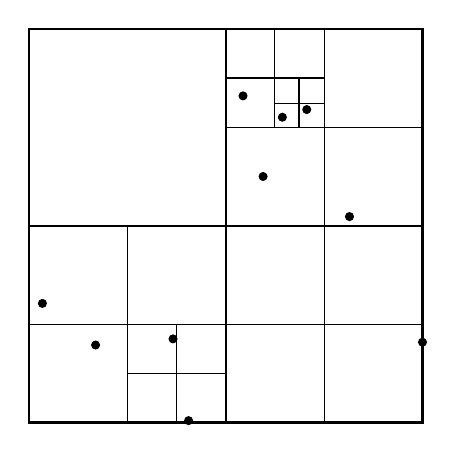
\begin{tikzpicture}[scale=0.05,%
		every circle node/.style = {width=3,fill=black}]
		
% Simulation domain
\draw[thick] (0,0) rectangle (100,100);
\pause
% Level 1
\draw[thick] (50,0) -- (50,100);
\draw[thick] (0,50) -- (100,50);
\draw[fill] (16.9664,19.6802) circle (1); %0
\pause
\draw[fill] (54.4110,82.9573) circle (1); %1
\pause
\draw (0,25) -- (50,25);
\draw (25,0) -- (25,50);
\draw[fill] (03.4614,30.2489) circle (1); %2
\pause
% Level 2
\draw (0,25) -- (100,25);
\draw (75,0) -- (75,100);
\draw (25,0) -- (25,50);
\draw (50,75)-- (100,75);
% Level 3
\draw (25,12.5) -- (50,12.5);
\draw (37.5,0)  -- (37.5,25);
\draw (62.5,75) -- (62.5,100);
\draw (50,87.5) -- (75,87.5);
% Level 4
\draw[thin] (68.625,75) -- (68.625,87.5);
\draw[thin] (62.5,81.125) -- (75,81.125);
% Particles (by increasing id)
\draw[fill] (81.4564,52.3018) circle (1); %3
\draw[fill](59.5102,62.4865) circle (1);  %4
\draw[fill] (40.5800,00.4751) circle (1); %5
\draw[fill] (64.4035,77.5371) circle (1); %6
\draw[fill] (36.6343,21.2396) circle (1); %7
\draw[fill] (99.9970,20.3979) circle (1); %8
\draw[fill] (70.6045,79.4802) circle (1); %9
		\end{tikzpicture}
		\caption{Sample 4-level Barnes-Hut grid with 10 particles.}
		\label{fig:bh-grid}
	\end{figure}
\end{frame}

\begin{frame}
	\frametitle{The Barnes-Hut Approximation: Tree Construction (Cont.)}
	\begin{figure}
		\centering
		\newlength{\lvld}
		\setlength{\lvld}{7em}
		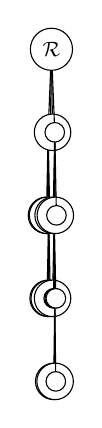
\begin{tikzpicture}[level distance=3em,
		sibling distance=3em,
		level 1/.style={sibling distance=0.80\lvld},
		level 2/.style={sibling distance=0.40\lvld},
		level 3/.style={sibling distance=0.4\lvld},
		level 4/.style={sibling distance=0.25\lvld},
		every node/.style = {shape=circle, draw, align=center, color=black,
			fill=white, scale=0.75}]
		\node {$\mathcal{R}$} %Root
child { node {} %1SW
	child { node{0} } %2SW
	child { node{2} } %2NW
	child { node{} %2SE
		child { node{} } %3SW
		child { node{7} } %3NW
		child { node{5} } %3SE
		child { node{} } } %3NE
	child { node{} } } %2NE
child { node{} }%1NW
child { node{8} }%1SE
child { node{} %1NE
	child { node{4} } %2SW
	child { node{} %2NW
		child { node {1} } %3SW
		child { node {} } %3NW
		child { node {} %3SE
			child { node{6} } %4SW
			child { node{} } %4NW
			child { node{9} } %4SE
			child { node{} } %4SW
		}
		child { node {} } }%3NE
	child { node{3} } %2SE
	child{ node{} } }; %2NE
		\end{tikzpicture}
		\caption{Tree structure associated to the configuration depicted in \cref{fig:bh-grid}.}
		\label{fig:bh-tree}
	\end{figure}
\end{frame}

\begin{frame}
	\frametitle{The Barnes-Hut Approximation: Force Computation}
	\begin{figure}
		\centering
		\begin{tikzpicture}[scale=0.035,%
		every circle node/.style = {width=3,fill=black}]
			% Simulation domain
\only<1,3->{\draw[thick] (0,0) rectangle (100,100);}
\only<2>{\draw[thick,fill=red!20!white] (0,0) rectangle (100,100);}
% Level 1
\draw[thick] (50,0) -- (50,100);
\draw[thick] (0,50) -- (100,50);
\only<3>{\draw[thick,fill=red!20!white] (0,0) rectangle (50,50);}
\only<12>{\draw[thick,fill=red!20!white] (0,50) rectangle (50,100);}
\only<13>{\draw[thick,fill=green!20!white] (50,0) rectangle (100,50);}
\only<14>{\draw[thick,fill=green!20!white] (50,50) rectangle (100,100);}
% Level 2
\draw (0,25) -- (100,25);
\draw (75,0) -- (75,100);
\draw (25,0) -- (25,50);
\draw (50,75)-- (100,75);
\only<4>{\draw[fill=red!20!white] (0,0) rectangle (25,25);}
\only<5>{\draw[fill=green!20!white] (0,25) rectangle (25,50);}
\only<6>{\draw[fill=red!20!white] (25,0) rectangle (50,25);}
\only<11>{\draw[fill=red!20!white] (25,25) rectangle (50,50);}
% Level 3
\draw (25,12.5) -- (50,12.5);
\draw (37.5,0)  -- (37.5,25);
\draw (62.5,75) -- (62.5,100);
\draw (50,87.5) -- (75,87.5);
\only<7>{\draw[fill=red!20!white] (25,0) rectangle (37.5,12.5);}
\only<8>{\draw[fill=green!20!white] (25,12.5) rectangle (37.5,25);}
\only<9>{\draw[fill=green!20!white] (37.5,0) rectangle (50,12.5);}
\only<10>{\draw[fill=red!20!white] (37.5,12.5) rectangle (50,25);}
% Level 4
\draw[thin] (68.625,75) -- (68.625,87.5);
\draw[thin] (62.5,81.125) -- (75,81.125);
% Particles (by increasing id)
\draw[fill=red] (16.9664,19.6802) circle (1); %0
\draw[fill] (54.4110,82.9573) circle (1); %1
\draw[fill] (03.4614,30.2489) circle (1); %2
\draw[fill] (81.4564,52.3018) circle (1); %3
\draw[fill](59.5102,62.4865) circle (1);  %4
\draw[fill] (40.5800,00.4751) circle (1); %5
\draw[fill] (64.4035,77.5371) circle (1); %6
\draw[fill] (36.6343,21.2396) circle (1); %7
\draw[fill] (99.9970,20.3979) circle (1); %8
\draw[fill] (70.6045,79.4802) circle (1); %9
		\end{tikzpicture}
		\hspace*{5pt}
		\setlength{\lvld}{4em}
		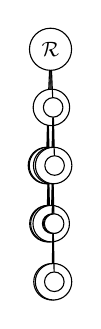
\begin{tikzpicture}[scale=0.7,
		level distance=3em,
		sibling distance=3em,
		level 1/.style={sibling distance=0.90\lvld},
		level 2/.style={sibling distance=0.50\lvld},
		level 3/.style={sibling distance=0.5\lvld},
		level 4/.style={sibling distance=0.4\lvld},
		every node/.style = {shape=circle, draw, align=center, color=black,
			fill=white, scale=0.75}]
		\node[onslide=<2>{coarse}]{$\mathcal{R}$}%Root
child { node[onslide=<3>{coarse}]{} %1SW
	child { node[onslide=<4>{coarse}]{0} } %2SW
	child { node[onslide=<5>{detail}]{2} } %2NW
	child { node[onslide=<6>{coarse}]{} %2SE
		child { node[onslide=<7>{coarse}]{} } %3SW
		child { node[onslide=<8>{detail}]{7} } %3NW
		child { node[onslide=<9>{detail}]{5} } %3SE
		child { node[onslide=<10>{coarse}]{} } } %3NE
	child { node[onslide=<11>{coarse}]{} } } %2NE
child { node[onslide=<12>{coarse}]{} }%1NW
child { node[onslide=<13>{detail}]{8} }%1SE
child { node[onslide=<14>{detail}]{} %1NE
	child { node{4} } %2SW
	child { node{} %2NW
		child { node {1} } %3SW
		child { node {} } %3NW
		child { node {} %3SE
			child { node{6} } %4SW
			child { node{} } %4NW
			child { node{9} } %4SE
			child { node{} } %4SW
		}
		child { node {} } }%3NE
	child { node{3} } %2SE
	child{ node{} } }; %2NE
		\end{tikzpicture}
		\caption{Hypothetical force computation for one particle of the system, \cref{fig:bh-grid,fig:bh-tree}.}
		\label{fig:bh-grid-forces}
	\end{figure}
\end{frame}

\begin{frame}
\frametitle{The Barnes-Hut Approximation: Tree Update}
\begin{figure}
	\centering
	\begin{tikzpicture}[scale=0.035,%
	every circle node/.style = {width=3,fill=black}]
	
% Simulation domain
\draw[thick] (0,0) rectangle (100,100);
% Level 1
\draw[thick] (50,0) -- (50,100);
\draw[thick] (0,50) -- (100,50);
\only<3>{\draw[detail] (0,0) rectangle (50,50);}
% Level 2
\draw (0,25) -- (100,25);
\draw (75,0) -- (75,100);
\draw (25,0) -- (25,50);
\draw (50,75)-- (100,75);
\only<2>{\draw[coarse] (0,0) rectangle (25,25);}
\only<4>{\draw[detail] (25,0) rectangle (50,25);}
% Level 3
\draw (25,12.5) -- (50,12.5);
\draw (37.5,0)  -- (37.5,25);
\draw (62.5,75) -- (62.5,100);
\draw (50,87.5) -- (75,87.5);
\only<5-6>{\draw[detail] (25,12.5) rectangle (37.5,25);}
% Level 4
\draw[thin] (68.625,75) -- (68.625,87.5);
\draw[thin] (62.5,81.125) -- (75,81.125);
\only<6->{%
\draw[thin] (31.625,12.5) -- (31.625,25);
\draw[thin] (25,18.625) -- (37.5,18.625);
}
\only<7>{\draw[detail] (25,18.625) rectangle (31.625,25);}
% Particles (by increasing id)
\only<1>{\draw[fill=red] (16.9664,19.6802) circle (1);} %0
\only<2->{\draw[fill=red] (26.9664,22.6802) circle (1);} %0
\draw[fill] (54.4110,82.9573) circle (1); %1
\draw[fill] (03.4614,30.2489) circle (1); %2
\draw[fill] (81.4564,52.3018) circle (1); %3
\draw[fill](59.5102,62.4865) circle (1);  %4
\draw[fill] (40.5800,00.4751) circle (1); %5
\draw[fill] (64.4035,77.5371) circle (1); %6
\draw[fill] (36.6343,21.2396) circle (1); %7
\draw[fill] (99.9970,20.3979) circle (1); %8
\draw[fill] (70.6045,79.4802) circle (1); %9
	\end{tikzpicture}
	\hspace*{5pt}
	\setlength{\lvld}{4em}
	\begin{tikzpicture}[scale=0.7,
	level distance=3em,
	sibling distance=3em,
	level 1/.style={sibling distance=0.90\lvld},
	level 2/.style={sibling distance=0.50\lvld},
	level 3/.style={sibling distance=0.5\lvld},
	level 4/.style={sibling distance=0.4\lvld},
	every node/.style = {shape=circle, draw, align=center, color=black,
		fill=white, scale=0.75}]
	\only<1-5>{%
\node {$\mathcal{R}$} %Root
child { node[onslide=<3>{detail}]{} %1SW
	child { node{0} } %2SW
	child { node[onslide=<2>{coarse}]{\only<1-5>{2}} } %2NW
	child { node[onslide=<4>{detail}]{} %2SE
		child { node{} } %3SW
		child { node[onslide=<5-6>{detail}]{7} } %3NW
		child { node{5} } %3SE
		child { node{} } } %3NE
	child { node{} } } %2NE
child { node{} }%1NW
child { node{8} }%1SE
child { node{} %1NE
	child { node{4} } %2SW
	child { node{} %2NW
		child { node {1} } %3SW
		child { node {} } %3NW
		child { node {} %3SE
			child { node{6} } %4SW
			child { node{} } %4NW
			child { node{9} } %4SE
			child { node{} } %4SW
		}
		child { node {} } }%3NE
	child { node{3} } %2SE
	child{ node{} } }; %2NE
}

\only<6->{%
\node {$\mathcal{R}$} %Root
child { node[onslide=<3>{detail}]{} %1SW
	child { node{0} } %2SW
	child { node[onslide=<2>{coarse}]{\only<1-6>{2}} } %2NW
	child { node[onslide=<4>{detail}]{} %2SE
		child { node{} } %3SW
		child { node[onslide=<5-6>{detail}]{}
			child { node{} } %4SW
			child { node[onslide=<7>{detail}]{\only<7>{2}} } %4NW
			child { node{} } %4SE
			child { node{7} } %4NE
		} %3NW
		child { node{5} } %3SE
		child { node{} } } %3NE
	child { node{} } } %2NE
child { node{} }%1NW
child { node{8} }%1SE
child { node{} %1NE
	child { node{4} } %2SW
	child { node{} %2NW
		child { node {1} } %3SW
		child { node {} } %3NW
		child { node {} %3SE
			child { node{6} } %4SW
			child { node{} } %4NW
			child { node{9} } %4SE
			child { node{} } %4SW
		}
		child { node {} } }%3NE
	child { node{3} } %2SE
	child{ node{} } }; %2NE
}
	\end{tikzpicture}
	\caption{Hypothetical tree update for one particle of the system, \cref{fig:bh-grid,fig:bh-tree}.}
	\label{fig:bh-grid-update}
\end{figure}
\end{frame}

\begin{frame}
	\frametitle{Data Structures}
	To compute forces, all we need is information about the centers of mass. In the code,
	\begin{itemize}
		\item A \lstinline{Particle} describes a center of mass (mass, position, velocity, acceleration).
		\item A \lstinline{Node} is a \lstinline{Particle} wrapper. It gives a center of mass information about its surrounding (geometrical boundaries, parent, children).
		\item A \lstinline{QuadTree} manages \lstinline{Node} objects. It provides methods to browse the tree.
		\item A \lstinline{Simulation} manages the run, times it (with \lstinline|Timer|) including IO (via \lstinline{IOManager}).
	\end{itemize}
\end{frame}

\begin{frame}
	\frametitle{Data Structures (Cont.)}
	\begin{figure}
		\centering
		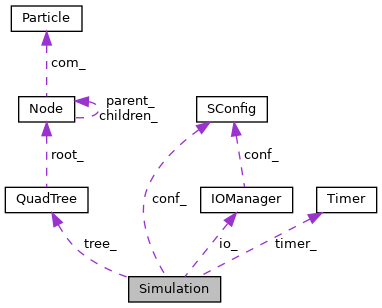
\includegraphics[width=0.5\textwidth]{inclfigs/class_simulation.png}
		\caption{Collaboration graph of the \lstinline|Simulation| class.}
	\end{figure}
\end{frame}

\begin{frame}
	\frametitle{Data Structures (Cont.)}
	Computation of the force should be the main task. Avoid memory latency issues if possible?
	\begin{itemize}
		\item<1-> SoA vs. \only<1>{AoS}\only<2->{\alert{AoS}}: SoA feasible on one CPU. However,
		\begin{itemize}
			\item Parallelized problem managing only some particles?
			\item Particles being passed after time evolution?
			\item Runaway particles?
		\end{itemize}
		\item<2-> \only<2>{Pointers}\only<3->{\alert{Pointers}} or array in the tree?
		\begin{itemize}
			\item Inhomogeneous particle distributions, most nodes empty.
			\item Using arrays means allocating full levels, exponentially increasing memory usage.
		\end{itemize}
	\end{itemize}

	\onslide<3->{However, the ``physical'' particles being simulated are kept local to another in a separate storage (in \lstinline|SConfig|).}
\end{frame}

\begin{frame}
	\frametitle{Recursion}
	All methods in the Barnes-Hut code avoid recursive calls.
	\begin{itemize}
		\item Much deeper levels possible for unbalanced problems. Stack could become large.
		\item More conditional statements, but also removes class inheritance (and thus virtual calls, vtables).
	\end{itemize}
\end{frame}

\begin{frame}
	\frametitle{Parallelization Strategy}
	\begin{itemize}
		\item Distribute \only<1>{only particles}\only<2>{\alert{only particles}}
		\begin{itemize}
			\item Minimal message size
			\item Instances need to rebuild their tree (and possibly query missing parts)
			\item Part of the work is duplicated on each process
		\end{itemize}
		\item Distribute the nodes
		\begin{itemize}
			\item Longer messages, especially for unbalanced problems
			\item Either compute prerequisites of each process or allow communicating missing parts
		\end{itemize}
	\end{itemize}
\end{frame}

\begin{frame}
\frametitle{Parallelization Strategy (Cont.)}
Particle sending/receiving:
\begin{itemize}
	\item Distribute all particles
	\begin{itemize}
		\item Minimal modifications to existing code
		\item After initial broadcast, only need to send ``managed'' particles
	\end{itemize}
	\item Distribute only managed particles
	\begin{itemize}
		\item Requires a \emph{tree completion} routine. Many short messages.
		\item Master thread or decentralized?
	\end{itemize}
\end{itemize}
\par
Particle ordering:~Already ordered along a ``multi-level'' Z-curve when we browse the leaf level. Distribute uniformly.
\par
Thread synchronization occurs when syncing leafs (\lstinline|MPI_Barrier| and \lstinline|MPI_Send/Recv|). %TODO-Fill
\end{frame}

\begin{frame}[fragile]
\frametitle{Parallelization Strategy (Cont.)}
Define a type for particles, \lstinline|MPI_Particle|.
	\begin{columns}
		\begin{column}{0.4\textwidth}
			\begin{figure}
				\centering
				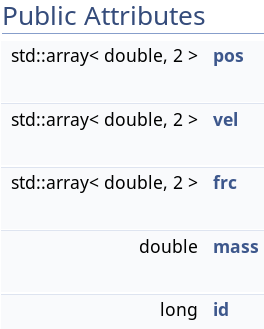
\includegraphics[width=\textwidth]{inclfigs/particle.png}
			\end{figure}
		\end{column}
		\begin{column}{0.6\textwidth}
			\lstinline|sizeof(double)=|\SI{8}{\byte}, \lstinline|sizeof(long)=|\SI{4}{\byte}.
	\end{column}
	\end{columns}
\end{frame}
	% ------------------ %
	\section{Performance}

\begin{frame}[fragile]
	\frametitle{TODO}
	Benchmarks run with
\begin{lstlisting}
npart=1000000
tevol_dt=0.00100000000
theta=0.400000
max_iter=20
\end{lstlisting}
	Compiled with \lstinline|O3|.
\end{frame}

\begin{frame}
	\frametitle{Hotspots}
	
\end{frame}

\begin{frame}
\frametitle{Bottom-Up}

\end{frame}

\begin{frame}
\frametitle{CPU Time}

\end{frame}
	% ------------------ %
	\section{Wrap-Up}
\subsection{Main Implementation Features}
\begin{frame}
	\frametitle{Strengths and Caveats: Serial}
\end{frame}

\begin{frame}
\frametitle{Strengths and Caveats: Parallel}
\end{frame}

\begin{frame}
\frametitle{Improvements}
\end{frame}
	% ------------------ %
	\begin{frame}[standout]
		Questions?
	\end{frame}
	\begin{frame}[t,allowframebreaks]
		\frametitle{References}
		\renewcommand{\bibfont}{\normalfont\footnotesize}
		\printbibliography[heading=none]
	\end{frame}
	% ------------------ %
	% Top secret section with extra material for a possible FAQ session at the end.
\appendix

\begin{frame}
	\frametitle{Problems affecting the code}
	\begin{itemize}
		\item When computing a leaf's interaction with a center of mass in an upstream branch (in which the leaf is located), the leaf's contribution to the upstream center of mass is not removed (that is, self-interaction occurs).
	\end{itemize}
\end{frame}

\begin{frame}
\frametitle{Why ``SuRMISe''}
\textbf{Surmise} \footcite{surmise}
\begin{quote}
	to guess something, without having much or any proof
\end{quote}
\par
\vspace{1cm}
Also the acronym for ``\alert{Su}rely \alert{R}uining \alert{M}y \alert{I}mpossible \alert{Se}mester''.
\end{frame}
\end{document}